\chapter*{Task 1}
\addcontentsline{toc}{chapter}{Task 1}

Task 1 requires computing two equilibrium points for the system, defining a reference curve between them. Then, it is required to compute an optimal trajectory to move from one equilibrium to another using the Newton's-like algorithm.

In general, the equilibrium points are all the points that satisfy the equation:

\begin{equation}
    x_{e} = f_{dis}(x_e,u_e)
\end{equation}

In our case, the discrete dynamics are the one described in (\ref{Discretized traj}), so a condition for equilibrium becomes that:

\begin{equation}
    x_e = x_e + f(x_e,u_e)\Delta t \longrightarrow f(x_e,u_e) = 0
\end{equation}

That means that the equilibrium points for the discrete dynamics are equal to those of the continuous dynamics.

Since the second joint is not controlled, the system is in equilibrium only if the second joint is in equilibrium. As we know for a simple pendulum, the equilibrium configurations are the ones where the absolute angle $\theta$ with respect to the world frame is equal to 0 or $\pi$. The world frame is defined such that the $y$ axis is parallel to the gravity vector and it is equal to the frame of joint one. So, we have that the second link is in equilibrium for each value of $q_2$ such that $q_1 + q_2 = 0 \text{ or } \pi$.

So, for the whole system, we have equilibrium when the velocities are zero, the input compensates for the gravity in the first joint (\ref{eq input}), and the second joint satisfies the equation $q_1 + q_2 = 0 \text{ or } \pi$.

\begin{equation} \label{eq input}
    u = G_1(q)
\end{equation}

Once two equilibrium points have been chosen, it is necessary to run the Newton's-like method with an initial guess that is a valid trajectory of the system. For our purposes, in task 1, we initialize the initial guess as constant vectors in the chosen initial equilibrium configuration.

The cost function is defined as follows:

\begin{equation}\label{Cost function}
\begin{aligned}
        \ell(x,u) = \sum_{t=0}^{T-1} (x_t - x_t^{ref})^TQ_t(x_t - x_t^{ref}) + (u_t-u_t^{ref})^TR_t(u_t-u_t^{ref})\\
        + (x_T - x_T^{ref})^TQ_T(x_T - x_T^{ref})
\end{aligned}
\end{equation}

and the unconstrained optimal control problem is stated as:

\begin{equation}
    \begin{aligned}
        &\min_{x \hspace{0.1cm}u} \hspace{0.1cm}\ell(x,u) \\
        &subj. to \hspace{0.5cm} x_{t+1} - f_d(x_t,u_t) = 0
    \end{aligned}
\end{equation}

The cost is a quadratic function of the states and the inputs. The Newton's-like method solves at each iteration a convex quadratic approximation of the whole problem, computing the descent direction as the solution of the Linear Quadratic Regulator.

The optimization is solved by considering an augmented state vector with the corresponding augmented matrices.

\begin{equation*}
    \Delta\Tilde{x}_t := \begin{bmatrix}
        1 \\
        \Delta x_t\end{bmatrix} 
\end{equation*}

\begin{equation*}
        q_t = \nabla_1 \ell(x_t^k,u_t^k) = Q_t(x_t^k - x_t^{ref}) \quad r_t = \nabla_2 \ell(x_t^k,u_t^k) = R_t(u_t^k - u_t^{ref})
\end{equation*}
            
\begin{equation*}
    Q_t = \nabla_{11} \ell(x_t^k,u_t^k) \quad R_t = \nabla_{22} \ell(x_t^k,u_t^k)
\end{equation*}

\begin{equation*}
    \Tilde{Q}_t := \begin{bmatrix}
        0 & q_t^T\\
        q_t & Q_t
    \end{bmatrix} \hspace{0.3cm}
    \Tilde{S}_t := \begin{bmatrix}
        r_t & S_t
    \end{bmatrix} \hspace{0.3cm}
    \Tilde{R}_t := R_t \hspace{0.3cm}
    \Tilde{A}_t := \begin{bmatrix}
        1 & 0\\
        c_t & A_t
    \end{bmatrix} \hspace{0.3cm}
    \Tilde{B}_t := \begin{bmatrix}
        0\\
        B_t
    \end{bmatrix} \hspace{0.3cm}
\end{equation*}

Then the associated LQR problem can be solved using the Difference Riccati Equation (\ref{Diff ricc eq}) for the matrix $P$ and computing the optimal gain $\Tilde{K}^*$ \footnote{The * denotes an optimal result}. To solve the problem, we use a regularized Newton's-like method where the terms $\nabla_{11}f_d(x_t^k,u_t^k)$ and $\nabla_{22}f_d(x_t^k,u_t^k)$ are ignored. In this way, we are sure that the matrices $\Tilde{Q}_t$ and $\Tilde{R}_t$ are always positive (semi-\footnote{The matrix $Q_t$ must be semi-positive definite, the matrix $R_t$ must be positive definite}) definite.

\begin{equation}
    \begin{aligned}
    &\min_{\Delta x \Delta u} \sum_{t=0}^{T-1} 
    \frac{1}{2}\begin{bmatrix}
        \Delta\Tilde{x}_t \\
        \Delta u_t
    \end{bmatrix}^T
    \begin{bmatrix}
        \Tilde{Q}_t & \Tilde{S}_t^T\\
        \Tilde{S}_t & \Tilde{R}_t
    \end{bmatrix}
    \begin{bmatrix}
        \Delta\Tilde{x}_t \\
        \Delta u_t
    \end{bmatrix}+\frac{1}{2} \Delta\Tilde{x}_T^T\Tilde{Q}_T\Delta\Tilde{x}_T \\
    & s.t. \hspace{0.5cm} \Delta\Tilde{x}_{t+1} = \Tilde{A}_t\Delta\Tilde{x}_t + \Tilde{B}_t\Delta\Tilde{u}_t \quad t = 0,..,T-1
    \end{aligned}
\end{equation}

The Difference Riccati Equation (\ref{Diff ricc eq}) is solved by backward integration, with the initial condition $P_T = \Tilde{Q}_T$.

\begin{equation}
    \Tilde{K}_t^* = -(\Tilde{R}_t + \Tilde{B}_t^T P_{t+1} \Tilde{B}_t)^{-1}(\Tilde{S}_t + \Tilde{B}_t^T P_{t+1} \Tilde{A}_t)
\end{equation}

\begin{equation} \label{Diff ricc eq}
    P_t = \Tilde{Q}_t + \Tilde{A}_t^T P_{t+1} \Tilde{A}_t - K_t^{*T}(\Tilde{R}_t + \Tilde{B}_t^T P_{t+1} \Tilde{B}_t )K_t^* \quad t = T-1,...,0
\end{equation}

To solve the convex quadratic problem, a shooting approach is considered. The solution is computed for $\Delta u$, and then $\Delta x$ is obtained through forward integration of the linearized dynamics.

\begin{equation}
    \begin{aligned}
        &\Delta\Tilde{u}_t = \Tilde{K}_t^*\Delta\Tilde{x}_t\\
        &\Delta\Tilde{x}_{t+1} = \Tilde{A}_t\Delta\Tilde{x}_t + \Tilde{B}_t\Delta\Tilde{u}_t
    \end{aligned}
\end{equation}

Once the descent direction $\Delta u^k$ is computed, the global solution can be updated using a robustified feedback integration of the dynamics. The step size can be chosen fixed or computed using Armijo's rule. Armijo's method is also useful to understand if the actual solution $\Delta u^k$ is effectively a descent direction, and it helps to check if the linearization of the dynamics is correctly computed by checking if the line (\ref{red line}), parametrized by $\gamma$, is tangent to the current cost $\ell(x^k,u^k)$.

\begin{equation} \label{red line}
    y(\gamma) = J(u^k) + \gamma \nabla J(u^k)^T\Delta u^k
\end{equation}

The step size selection condition for Armijo's rule is

\begin{equation}
    J(u^k + \gamma\Delta u^k) \geq J(u^k) + \gamma \nabla J(u^k)^T\Delta u^k
\end{equation}

\begin{equation}
    \begin{aligned}
        &u_t^{k+1} = u_t^{k} + K_t^k(x_t^{k+1}-x_t^k) + \gamma^k\sigma_t^k\\
        & x_{t+1}^{k+1} = f_d(x_t^{k+1},u_t^{k+1})        
    \end{aligned}
\end{equation}

The algorithm stops the iterations when it finds a descent direction whose squared amplitude is lower than a certain threshold, or when Armijo's method fails to determine a feasible step size.

In our case, we have chosen the following equilibrium point:

\begin{equation*}
\begin{aligned}
    &x_{init} = [0,0,0,0] \\
    &x_{fin} = [90,-90,0,0]
\end{aligned}  
\end{equation*}

These points are easy to reach because they are stable. A step reference transition has been chosen (Fig \ref{fig:downward_0}). The simulation time is set to 10 seconds, and the discretization time is 0.01 seconds. 

The weights in the cost have been selected experimentally, and a good compromise resulted in:

\begin{equation*}
    \begin{aligned}
        &Q_t = \begin{bmatrix}
            1000 & 0 & 0 & 0 \\
            0 & 1000 & 0 & 0 \\
            0 & 0 & 10 & 0\\
            0 & 0 & 0 & 10
        \end{bmatrix} = Q_T\\
        &\\
    & R_t = 10
    \end{aligned}
\end{equation*}

The algorithm requires 8 iterations to converge to a solution. As shown in the descent direction figure (\ref{fig:Downward_Descent}), the value of the norm falls below $10^{-6}$, which is the value chosen for the threshold.

The Armijo parameters have been selected using the values from the course slides:

\begin{itemize}
    \item $\beta$ = 0.7
    \item  $c$ = 0.5
\end{itemize}

\begin{figure}
    \centering
    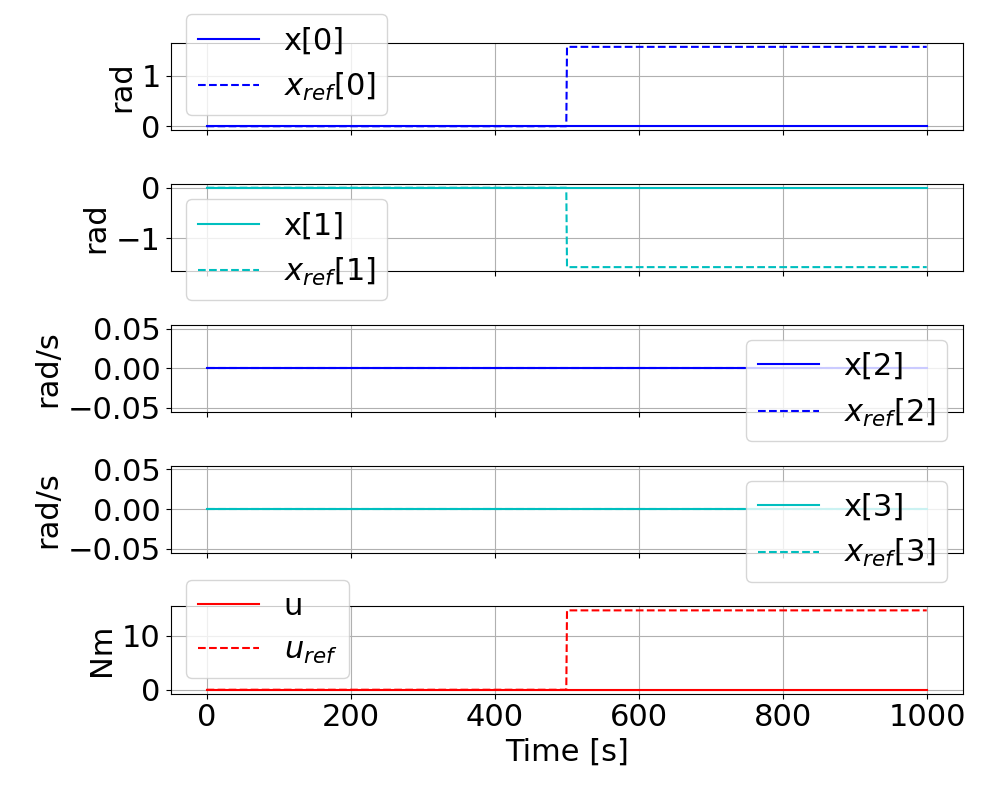
\includegraphics[width=0.8\linewidth]{figs/downwards_0.png}
    \caption{Reference and initial guess}
    \label{fig:downward_0}
\end{figure}

\begin{figure}
    \centering
    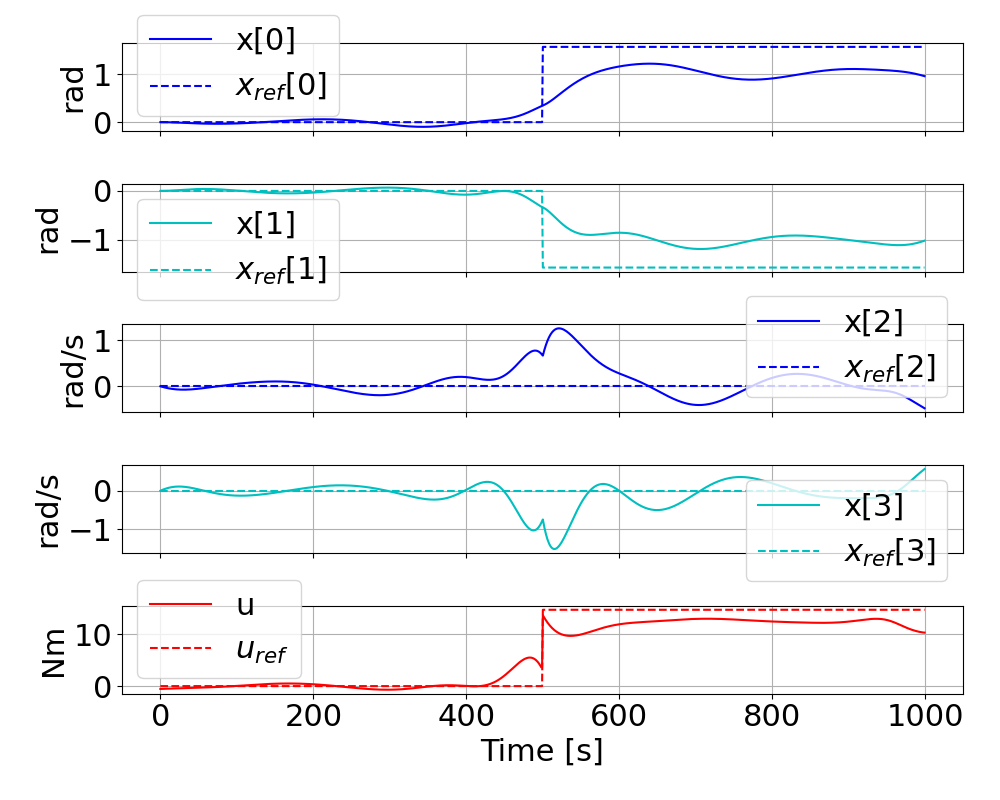
\includegraphics[width=0.8\linewidth]{figs/downwards_1.png}
    \caption{First iteration}
    \label{fig:downwards_1}
\end{figure}

\begin{figure}
    \centering
    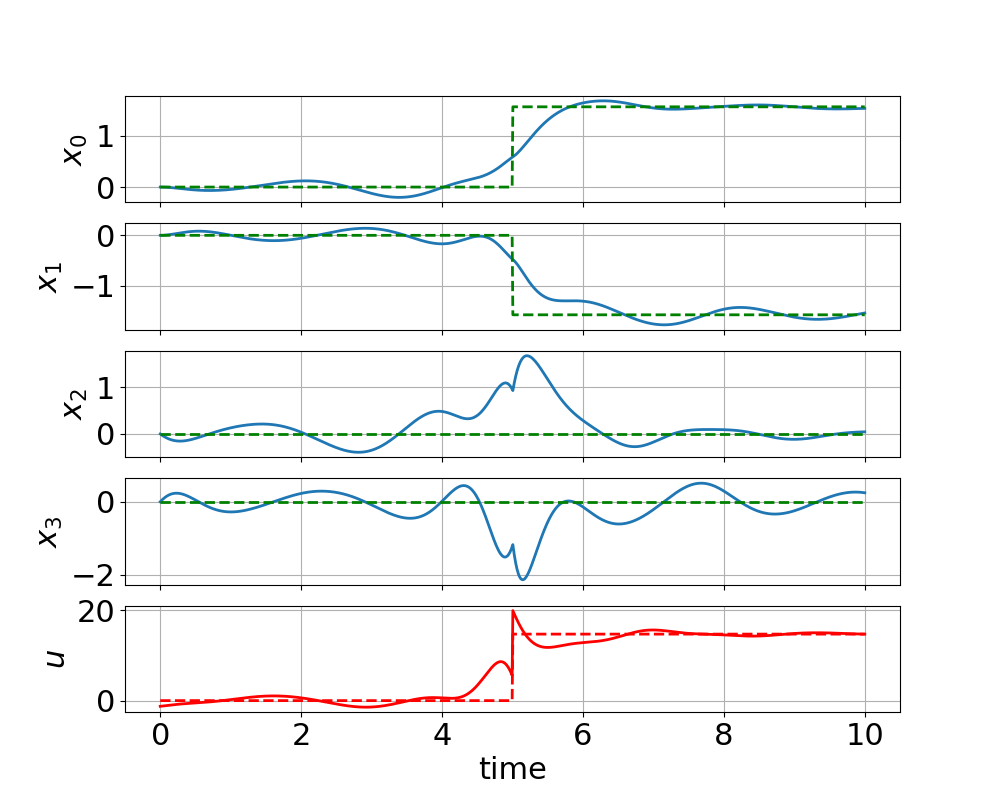
\includegraphics[width=0.8\linewidth]{figs/downwards_f.png}
    \caption{Final result}
    \label{fig:downward_f}
\end{figure}

\begin{figure}
    \centering
    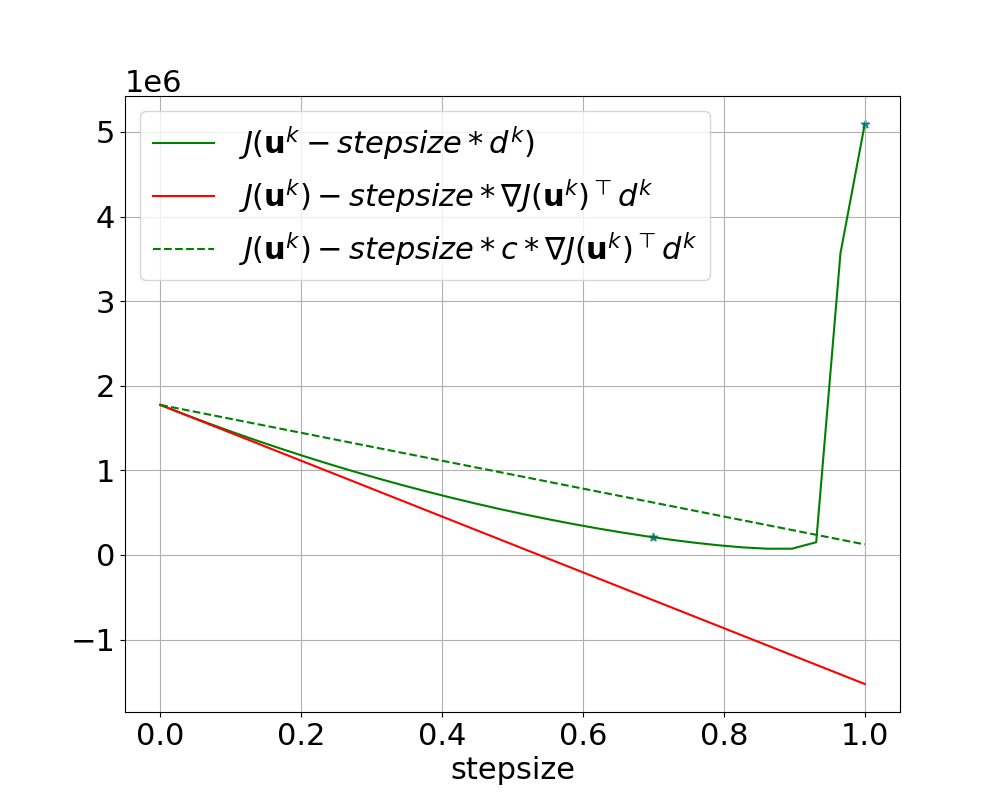
\includegraphics[width=0.8\linewidth]{figs/downward_armijio_0.png}
    \caption{Backtracking line search plot at the first iteration}
    \label{fig:downward_armijio_0}
\end{figure}

\begin{figure}
    \centering
    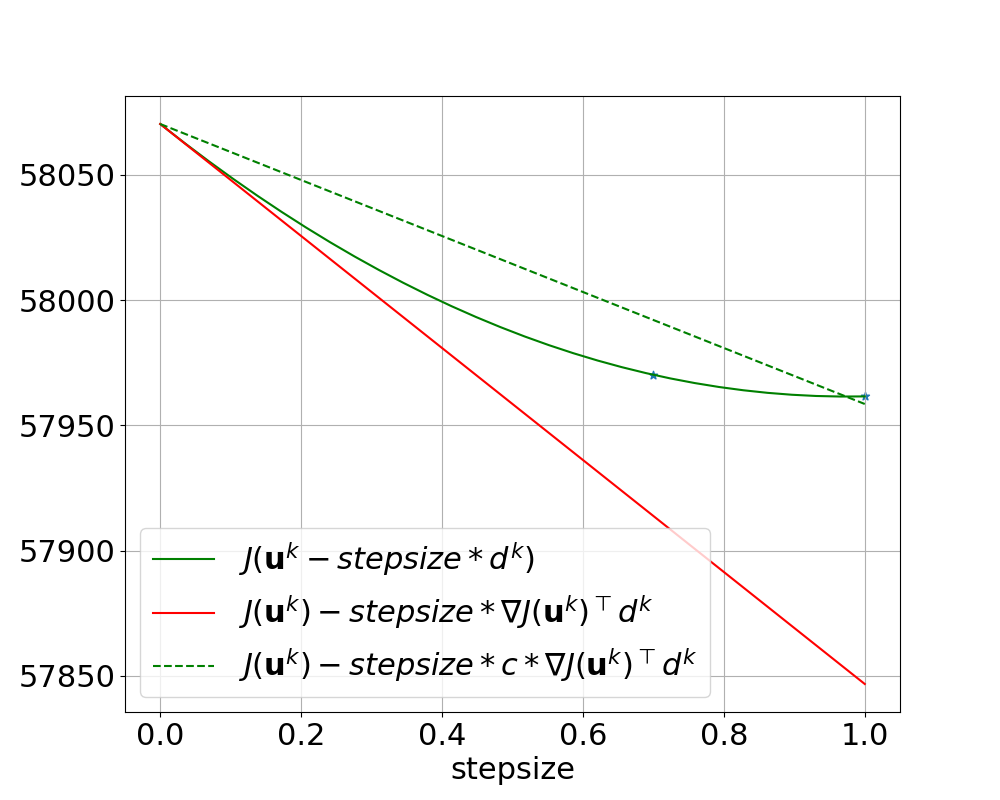
\includegraphics[width=0.8\linewidth]{figs/downward_armijio_3.png}
    \caption{Backtracking line search plot at the third iteration}
    \label{fig:downward_armijio_3}
\end{figure}

\begin{figure}
    \centering
    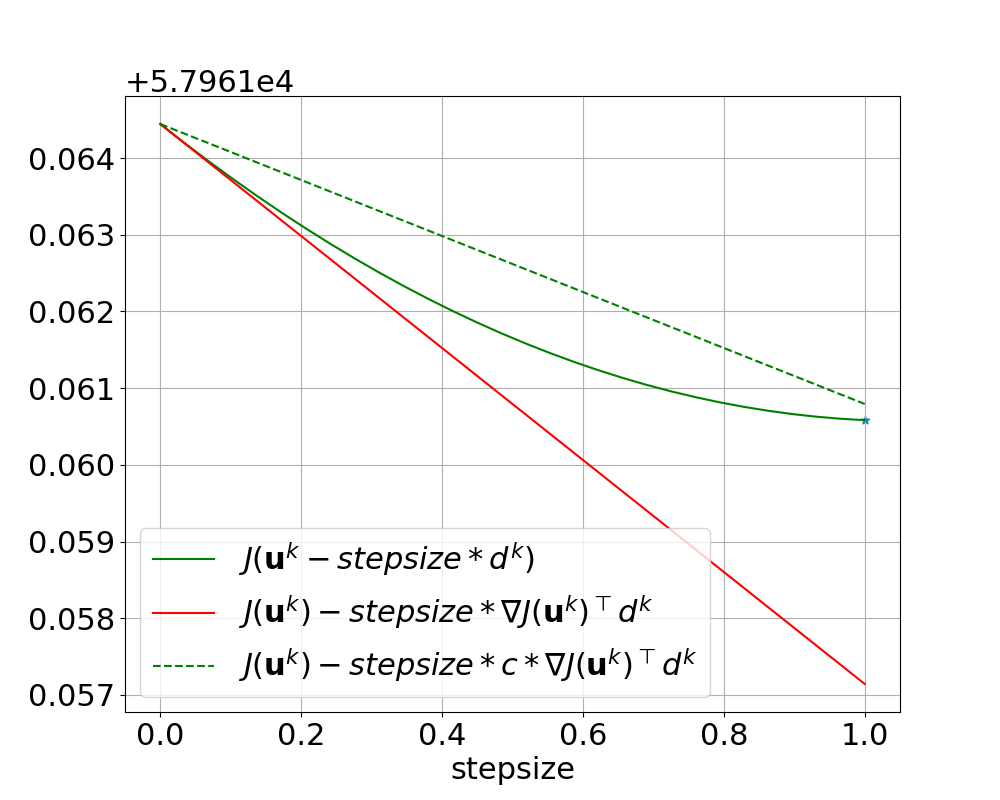
\includegraphics[width=0.8\linewidth]{figs/downward_armijio_6.png}
    \caption{Backtracking line search plot at the sixth iteration}
    \label{fig:downward_armijio_6}
\end{figure}

\begin{figure}[htbp]
    \centering
    \begin{subfigure}[b]{0.49\textwidth}
        \centering
        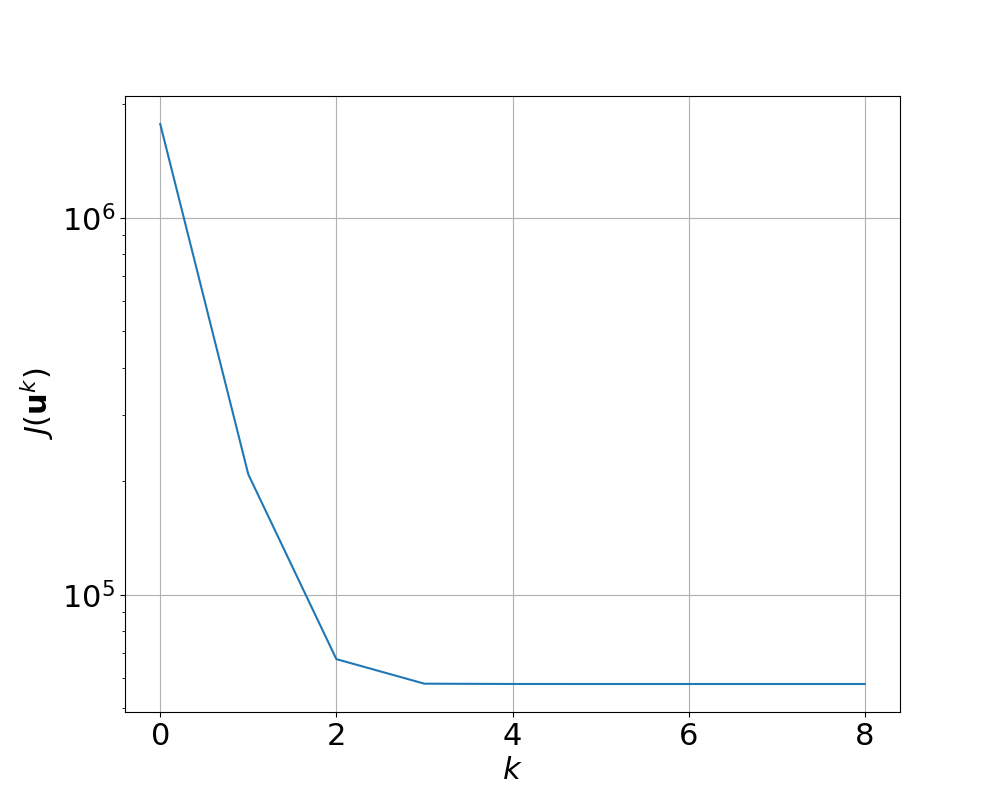
\includegraphics[width=\textwidth]{figs/downward_cost.png}
        \caption{Cost}
        \label{fig:downward_cost}
    \end{subfigure}
    \hfill
    \begin{subfigure}[b]{0.49\textwidth}
        \centering
        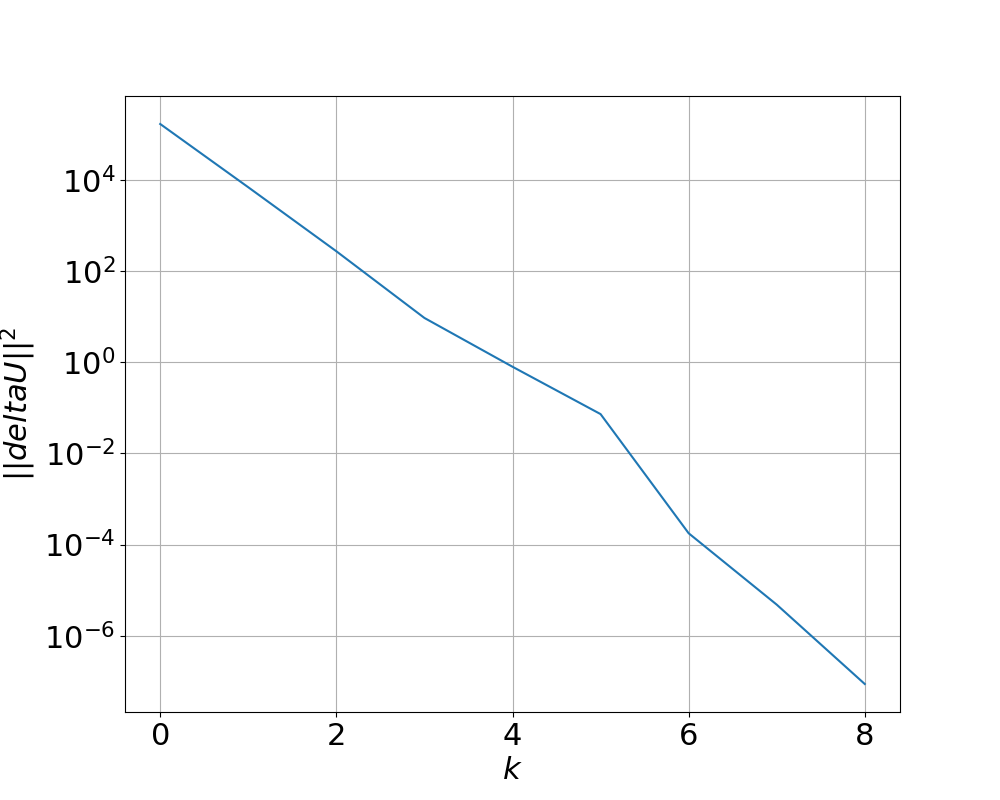
\includegraphics[width=\textwidth]{figs/Downward_Descent.png}
        \caption{Descent direction}
        \label{fig:Downward_Descent}
    \end{subfigure}
    \caption{}
\end{figure}

\section*{Python code}
The reference trajectory is defined in the Python file reference\_trajectory.py.

The Newton's method solver is defined in the Python file solver.py.

\begin{itemize}
    \item \textbf{step(xx\_init, xx\_fin, tf, dt) }Compute a step curve between xx\_init and xx\_fin. The input is calculated as the gravity compensation along the resulting state reference curve.\\\\
    \textbf{Arguments}:
    \begin{itemize}
        \item xx\_init : Initial state vector in degrees.
        \item xx\_fin : Final state vector in degrees.
        \item tf : Final time in seconds.
        \item dt : Time of dicretization in seconds.
    \end{itemize}
    \textbf{Return}:
    \begin{itemize}
        \item xx\_ref : Reference curve between the two states from 0 to tf, in radiants.
        \item uu\_ref : Input reference curve.
    \end{itemize}
    
    \item \textbf{step\_comp(points, tf, dt) }: Compute a composition of step curves between state configuration points. The input is calculated as the gravity compensation along the resulting state reference curve.\\\\
    \textbf{Arguments}:
    \begin{itemize}
        \item points : List of state vectors in degrees.
        \item tf : Final time in seconds.
        \item dt : Time of dicretization in seconds.
    \end{itemize}
    \textbf{Return}:
    \begin{itemize}
        \item xx\_ref : State reference curve in radiants.
        \item uu\_ref : Input reference curve.
    \end{itemize}

\item \textbf{newton\_solver(xx\_ref, uu\_ref, xx\_init, uu\_init, dyn, tf, dt, max\_iters, ...) }: Compute the optimal trajectory using the Newton's-like method. The Armijo's method is also implemented for the selection of the step size. \\\\
    \textbf{Arguments}:
    \begin{itemize}
        \item xx\_ref : Reference state curve.
        \item uu\_ref : Reference input curve.
        \item xx\_init : Initial guess state trajectory.
        \item uu\_init : Initial guess input trajectory.
        \item dyn : dynamic package imported from Dinamics.py.
        \item tf : Final simulation time, in seconds.
        \item dt : Time of dicretization in seconds.
        \item max\_iters : Maximum number of iteration of the algorithm.
        \item term\_cond = 1e-1 : Is the terminal condition for the squared magnitude of the discent direction.
        \item fixed\_stepsize = 1e-1 : Step size value if Armijio is not enabled.
        \item armijo = False : Armijo enable variable.
        \item dynamic\_plot = False : Plot while executing.
        \item visu\_descent\_plot = False : Armijio plot.
        \item armijo\_maxiters = 20 : Maximum number of iteration for the stepsize search.
        \item cc = 0.5 : Armijo paramiter.
        \item beta = 0.7 : rate of reduction of the stepsize at each armijo iteration.
        \item stepsize\_0 = 1 : Initial Armijo stepsize.
    \end{itemize}
    
    \textbf{Return}:
    \begin{itemize}
        \item xx\_star : Optimal State Trajectory.
        \item uu\_star : Optimal Input Trajectory.
        \item JJ : Vector of acquired costs.
        \item descent : Squared value of the magnitude of the descent direction.
        \item max\_iter : Number of effective iterations.
    \end{itemize}

\end{itemize}